\chapter{Identification d'appareils LoRa par la méthode des constellations traces figures}

Ce chapitre a pour but d'approfondir l'analyse des charactéristiques uniques des fréquences radios. Plutot que de s'intéresser au routine entre les communication ou la distance d'où elles ont lieu, le \textit{Radio Frequency Finguerprinting} se concentre sur les propriétés physiques des signaux. Différentes techniques sont montrées par N. Soltanieh, Y. Norouzi et Y. Yang\cite{rffi1}. L'approche principale choisie se base la méthode des \textit{differential constellations traces figures (DCTF)} developpé dans l'article \cite{loraDCTF} par Yu Jiang, Linning Peng, Aiqun Hu, Sheng Wang, Yi Huang et Lu Zhang. Dans un premier temps la méthode de l'article est présentée de manière théorique avant d'être appliquée sur les appareils afin de réaliser l'objectif du mémoire. Cependant, plusieurs modifications ont été ajoutées afin de pousser plus loin les possibilitées de la méthode.

\section{Radio Frequency Fingerprinting avec DCTF}\label{DCTF}

Cette section se base sur l'article \cite{loraDCTF}. L'objectif principale de la méthode consiste à révéler la signature radio d'un signal, permettant ainsi à partir de cette signature de retrouver l'appareil émetteur.

La méthode des diagrammes de constellations est une projection des échantillons I/Q dans le plan complexe. Cette projection permet en théorie d'extraire des features comme :

\begin{itemize}
\item des erreurs ou offset de fréquences. Cela peut être une déviation de la fréquence du signal par rapport à la fréquence attendue. Cela se représente sur le diagramme de constellation par un décalage des échantillons. 
\item Une mauvaise synchronisation. Si le récepteur est mal synchronisé (sur la phase, le temps ou encore la fréquence) cela peut faire apparaitre des distorsions sur le diagramme.
\item I/Q origin offset. Un décalage entre les composante I et Q peut provoquer un décalage des donnée par rapport à l'origine sur le diagramme de constellation.
\item Des erreurs de magnitude. Des variations sur l'amplitude du signal altèrent la densité du diagramme de constellation.
\end{itemize}

Ajouté à toutes ces possibles features, l'article mentionne la possibilités de trouver via le diagrame de constellations \textit{l'unique caractéristique physique du signal}. Cepepant cette caractéristique n'est pas immédiatement visible. L'influence de l'offset de fréquence fait dévier les symboles de leur positions originales, ce qui couvre l'information tout le long du diagramme de constellation.


idée: le received singal contient le baseband singal ainsi qu'un rotation factor instable. pour pouvoir recover cette partie du signal, besoin d'effctuer une opération différentielle suivante :

\begin{equation}\label{eq1}
	x(t) . x(t+n) e -j2\pi on
\end{equation} 

apparation d'un nouveau rotation factor, mais stable. Besoin de trouver deux inconnue,\textit{delta f} et \textit{n}. n est le differential interval. il se calcule de la manière suivante :

\begin{equation}\label{eq2}
 Rs = BW / 2sf \\
 N = fs / Rs
\end{equation}

carrier frequency offset :
\begin{equation}\label{eq3}
 CFO
\end{equation}

\section{Méthode DCTF en pratique}

L'analyse suivante est basée sur l'article publié  \cite{loraDCTF}. L'objectif de cette analyse est de pouvoir identifier un appareil LoRa uniquement en se fiant à l'analyse des signaux générés par ce dernier. 

Le signal test pour cette analyse est le signal contenant les paramètres suivants :

\vspace{0.1cm}

\begin{itemize}
\item émetteur : module RN2483, modulation : LoRa, SF = 8, BW = 125KHz, frequency = 868MHz, pwr = 14, cr = 4/8.
\item Récepteur : RTL SDR R820T2, f = 867,9375MHz, SR = 2MHz, gain = 5dB.
\end{itemize}

\vspace{0.1cm}

Ce signal a été normalisé avec \textit{Root Means Square}.



\begin{figure}[h]
\centering

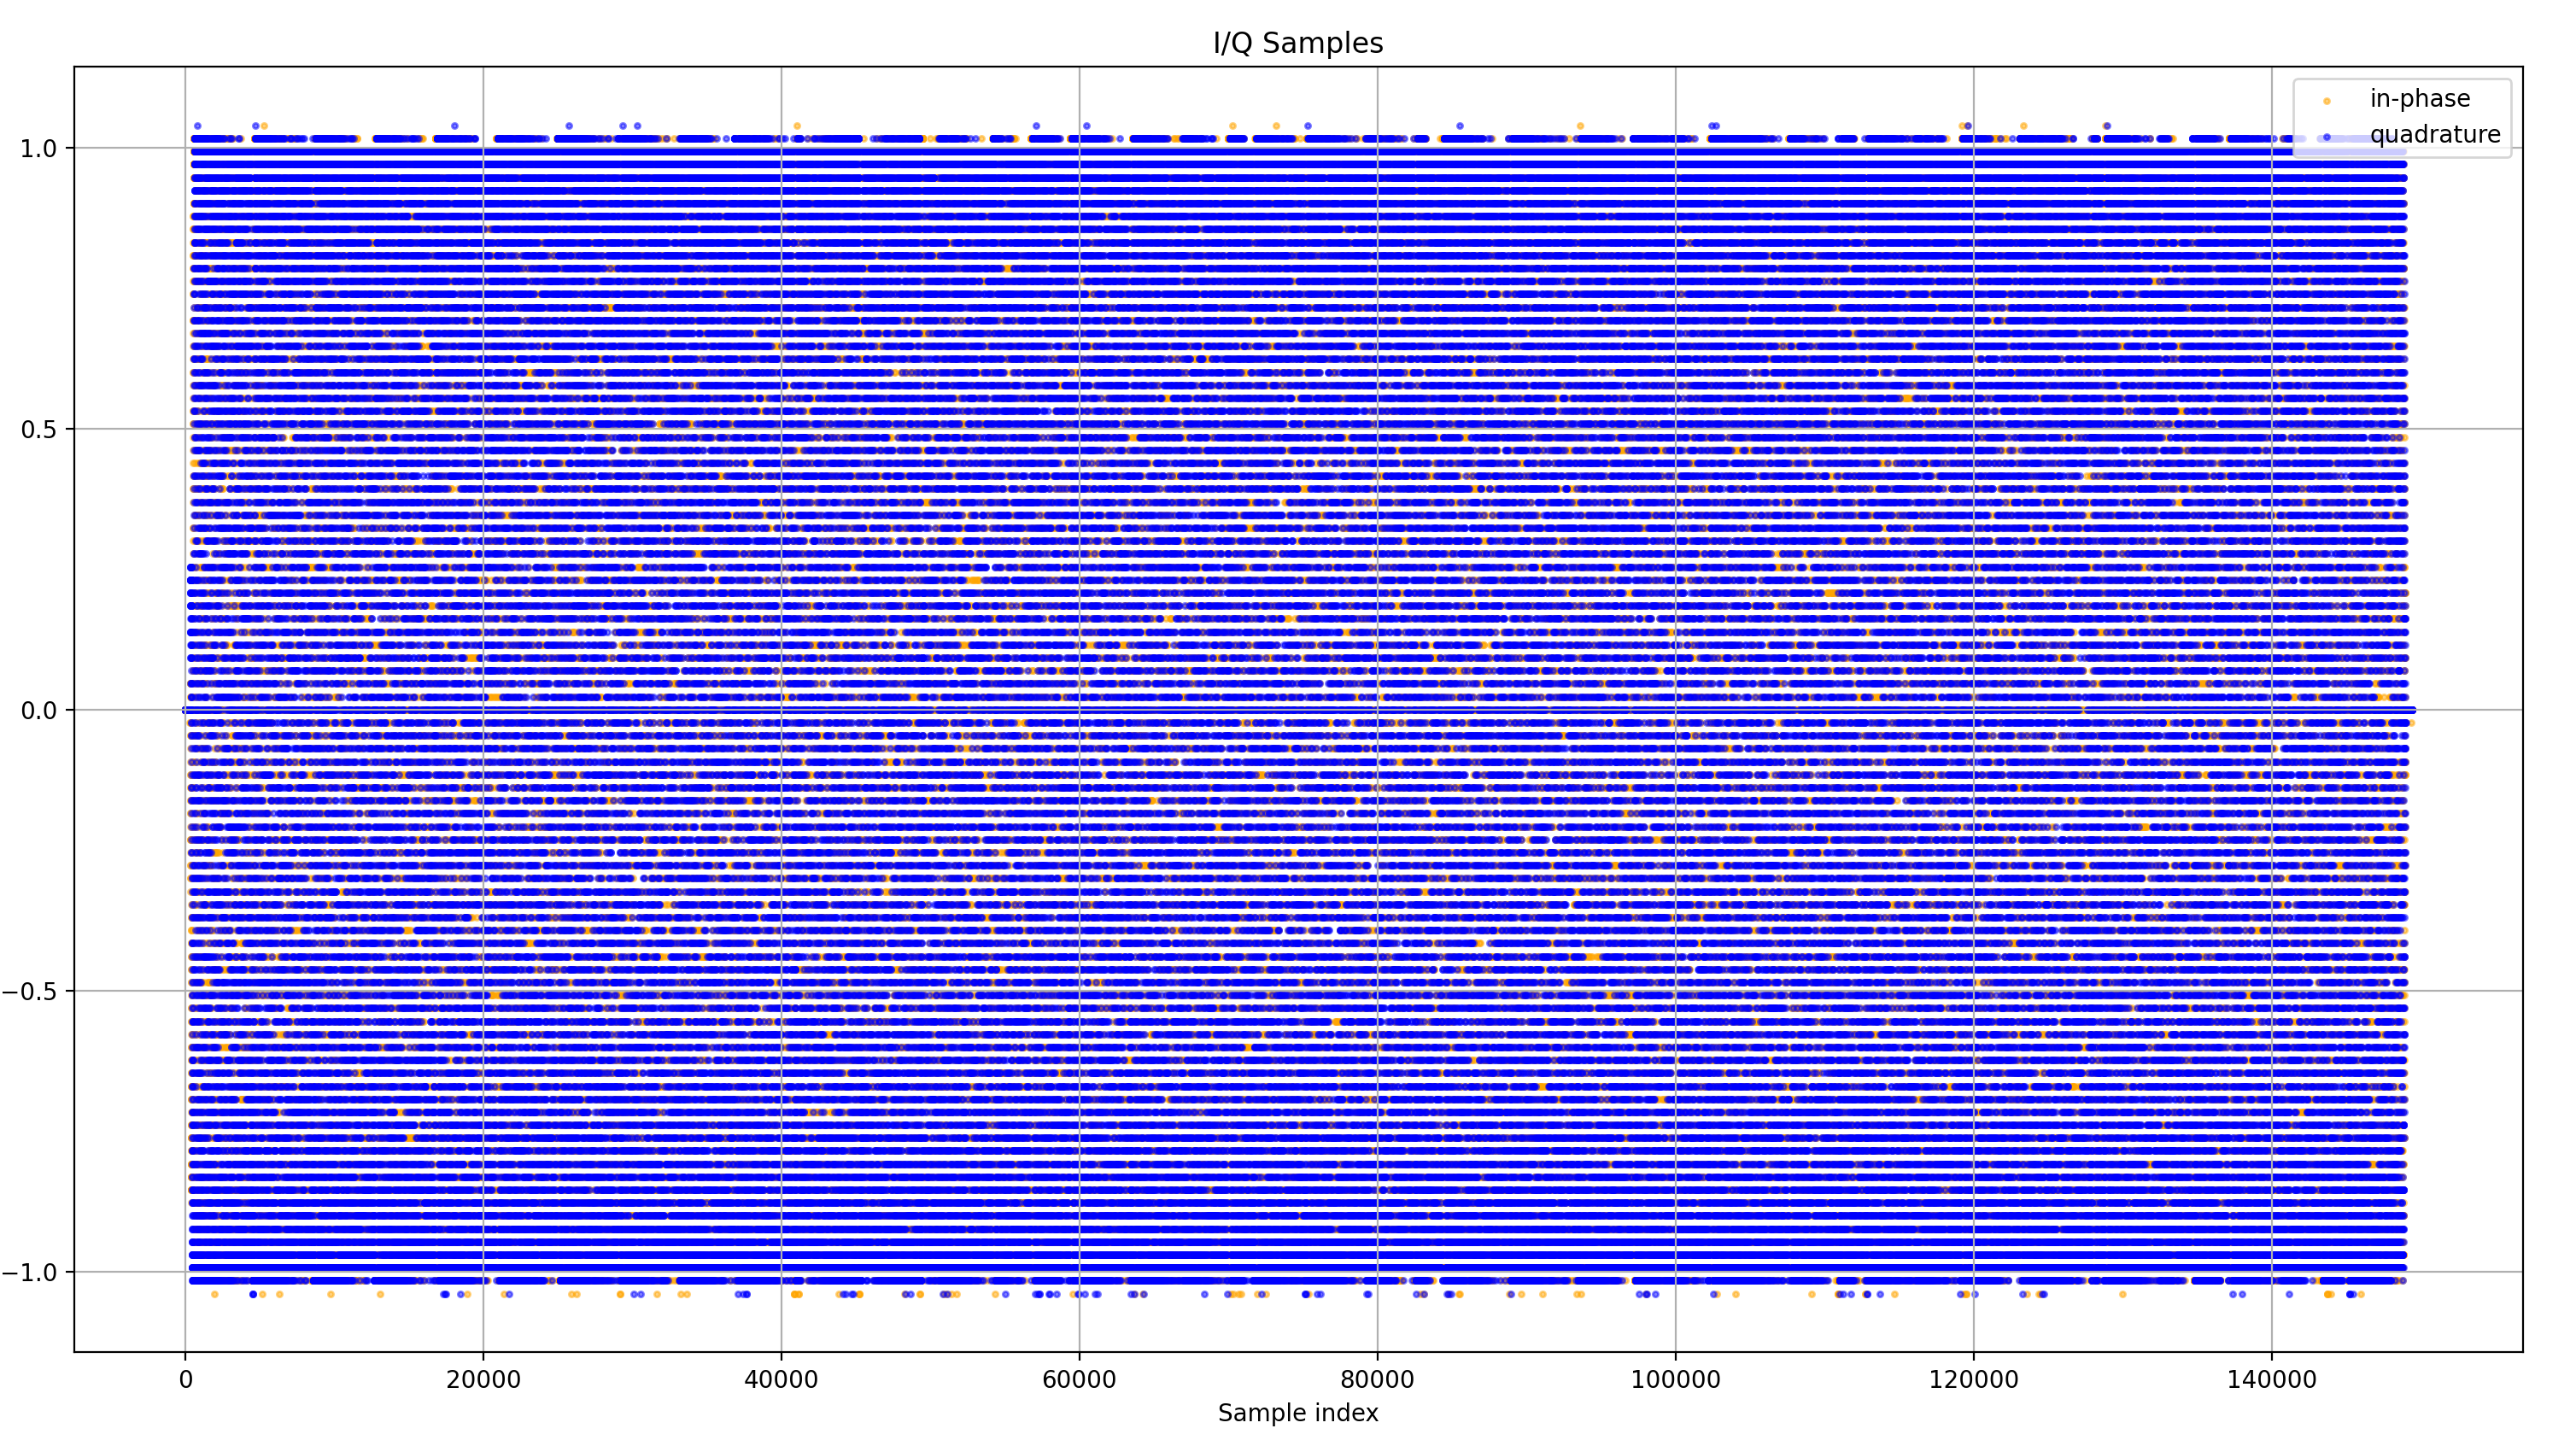
\includegraphics[scale=0.12]{images/dctf2.png}
\caption{LoRa signal}\label{term313}
\end{figure}


\begin{figure}[h]
\centering

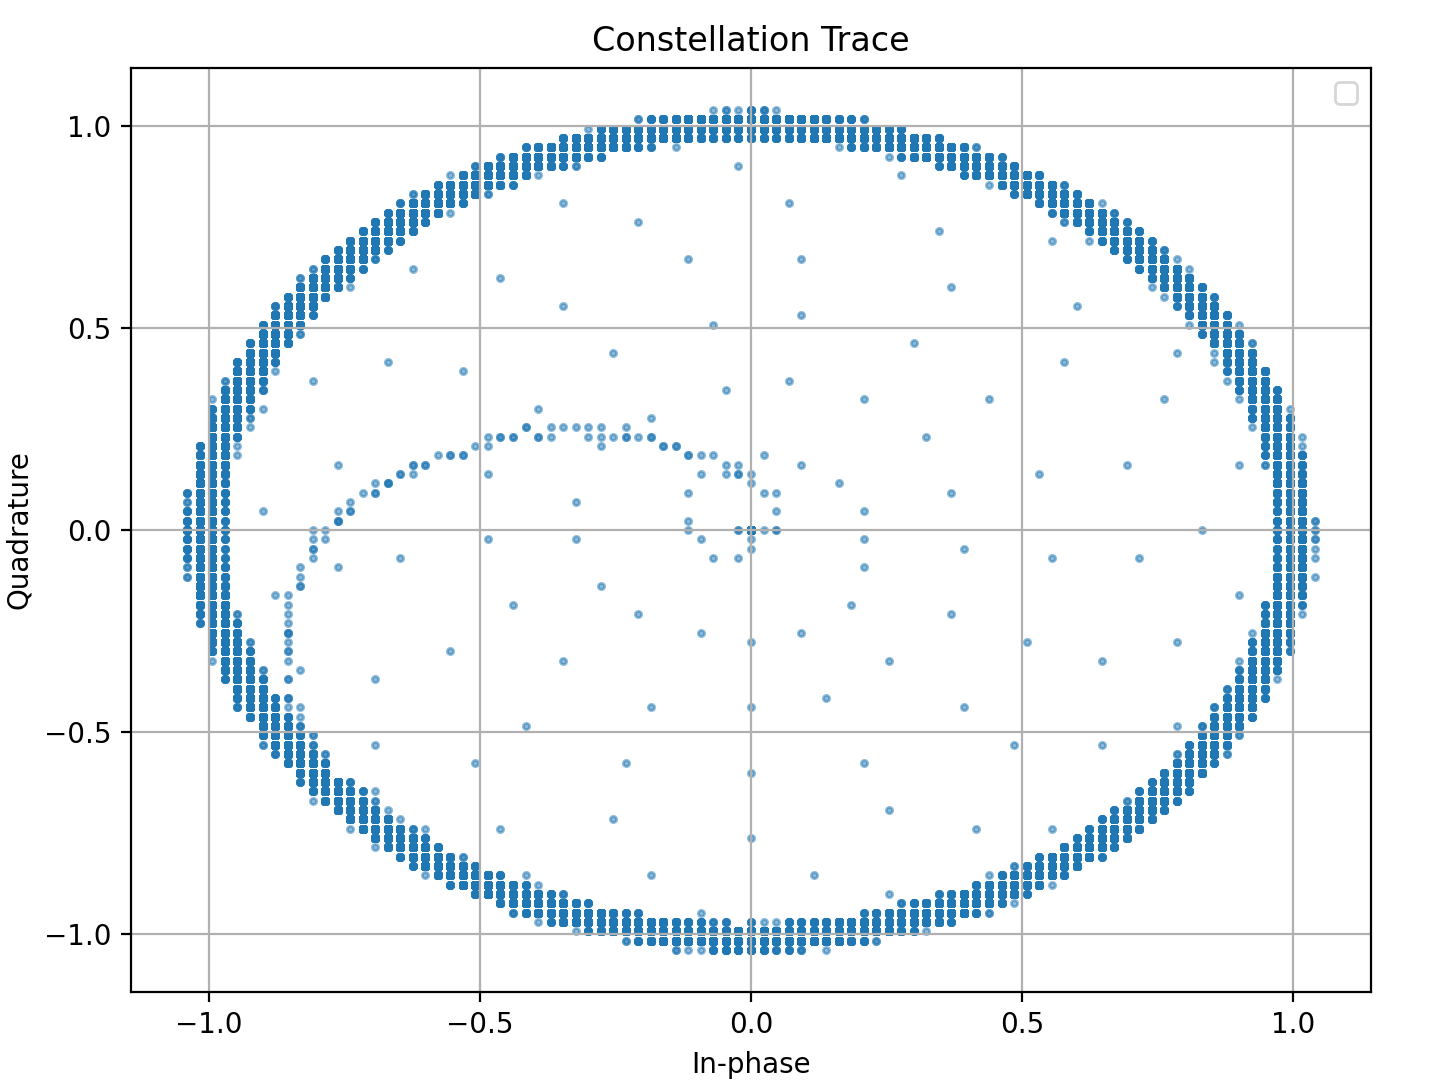
\includegraphics[scale=0.25]{images/dctf1.png}
\caption{Diagramme de constellation}\label{term314}
\end{figure}


La méthode DCTF se base sur l'utilisation de constellations traces pour pouvoir identifier sur base de propiétées uniques un appareil. Un diagramme de constellations est une représentation dans le plan complexe de la distribution spaciale des points du signal. La figure \ref{term313} montre la représentation dans le temps du signal test et sa représentation sous forme de constellation est donnée par la figure \ref{term314}.



Selon la section \ref{DTCF}, le diagramme de constellation seul n'est pas suffisant pour pouvoir identifier des composantes uniques au signal. Pour pouvoir observer l'émergence d'une signature, il faut appliquer la méthode différentielle décrite dans \ref{DCTF} ainsi que dans l'article \cite{loraDCTF}. La figure \ref{term316} montre le diagramme differentiel de constellation \textit{DCTF} du signal. L'équation \ref{eq1} possède deux paramètres à calculer. Le \textit{différential interval (N)} se calcule via \ref{eq2} et vaut 4096. Le \textit{Carrier Frequency Offset (CFO)} peut être estimé via \ref{eq3}. Dans un premier temps sa valeur est estimée à 0.

\begin{figure}[h]
\centering

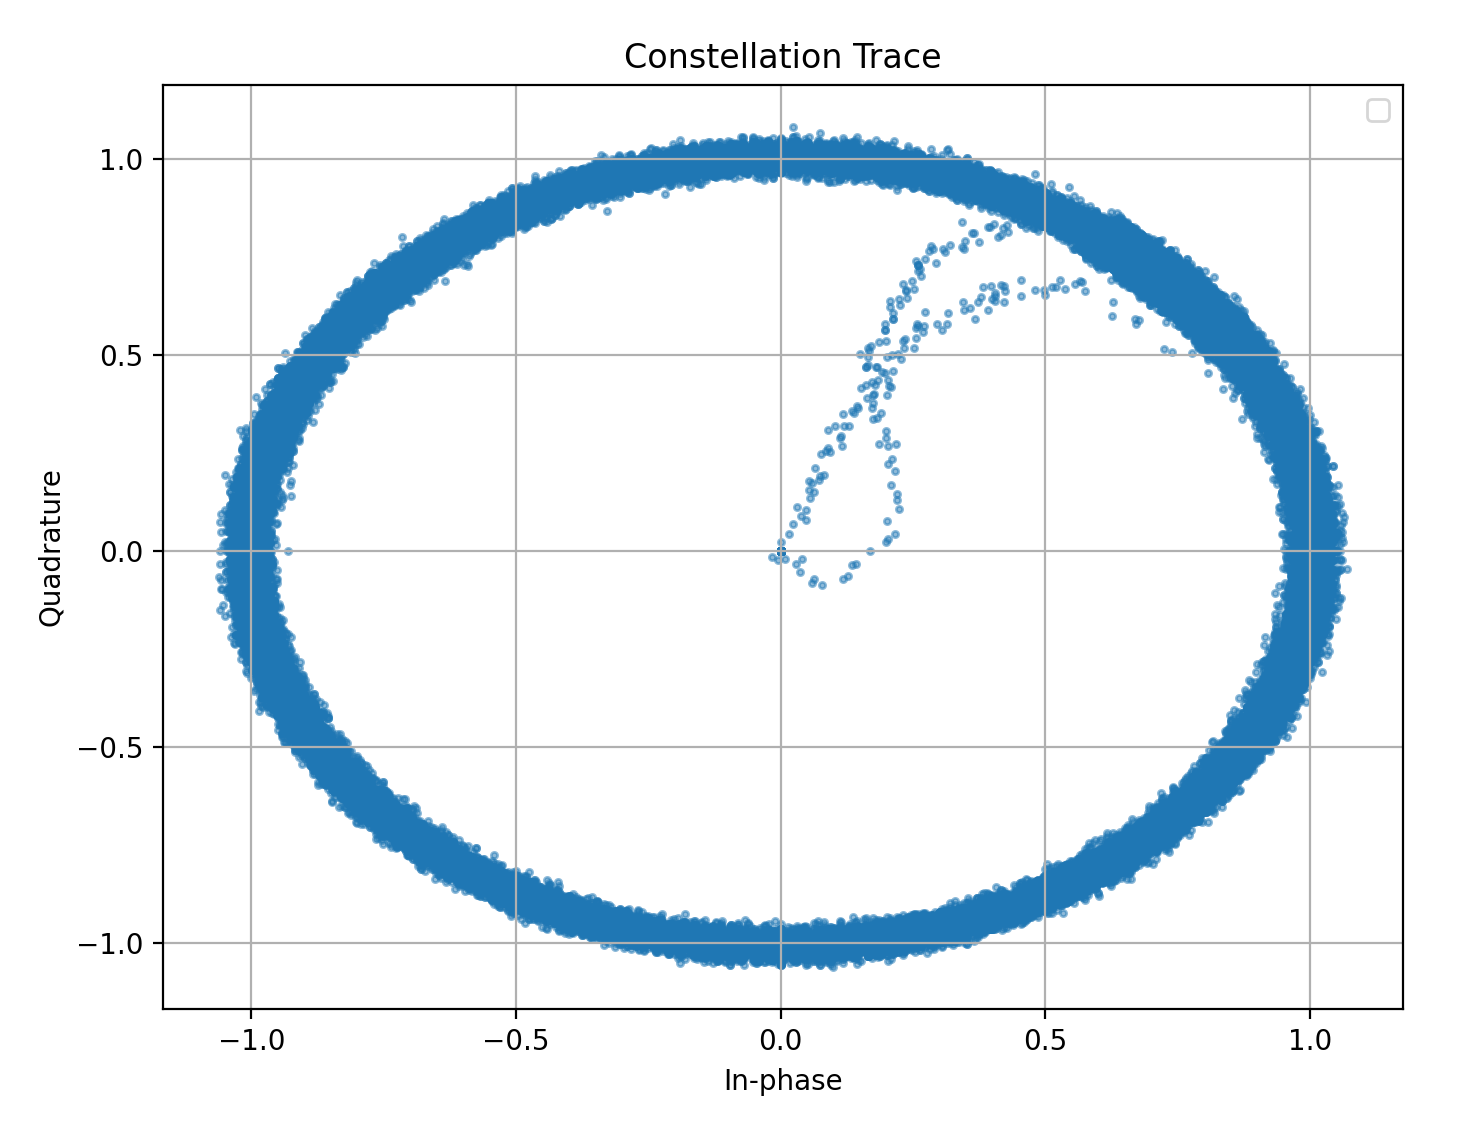
\includegraphics[scale=0.25]{images/dctf3.png}
\caption{DCTF du signal test}\label{term316}
\end{figure}

On remarque que la forme de la constellation est similaire, mais l'application de la méthode différentielle juxtapose les points les uns sur les autres à tel point qu'il devient difficile d'analyser en détail sa composition. Pour pouvoir observer une composante susceptible d'être une signature, il faut appliquer un gradient coloré pour évaluer la densité des points de la constellations. La figure \ref{term317} montre le même diagramme qu'à la figure \ref{term316} mais avec l'utilisation de la librairie python Datashader, qui ajoute une échelle de densité (en poucentage, ou 100 représente la zone la plus dense du diagramme). On observe que dans le coin supérieur droit la densité de point est un peu plus élevé que dans le reste de la constellation.

\begin{figure}[h]
\centering

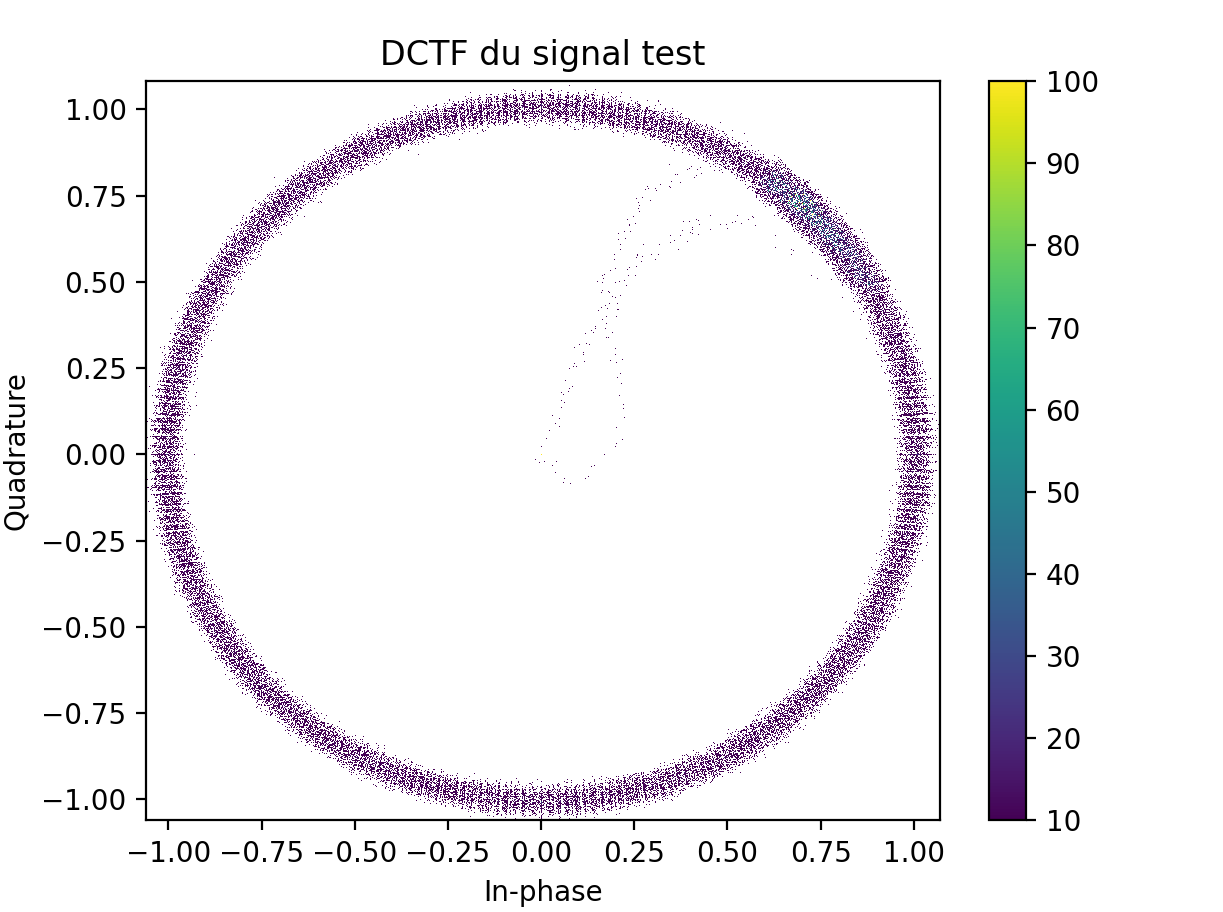
\includegraphics[scale=0.3]{images/dctf4.png}
\caption{DCTF du signal test}\label{term317}
\end{figure}

Jusqu'à présent, l'analyse a été faite en utilisant l'intégralité du signal comme donnée. Cependant l'article \cite{loraDCTF} a montré qu'il est possible de filtrer une partie des données et ainsi ne conserver qu'une partie suffisante du signal pour déterminer sa signature. Premièrement, d'un point de vue physique, le signal possède une partie appelée \textit{transient part}, c'est la portion initiale du signal qui contient la transition d'un état vers un autre. Cette partie se caractérise sur la figure \ref{term317} par les points qui ne se situent pas sur la constellation mais entre la constellation et le centre du plot. Dans ce domaine, cette partie concerne le moment ou le module s'enclenche, occasionant des irrégularités dans la réception des données. Cette partie seule étant instable, elle est écarté des données analysées. Ensuite, l'intégralité du signal n'est pas nécessaire. En effet, le contenu du message (dans la partie payload du paquet LoRa) est sujet à modifications et n'est pas pertinent pour l'analyse, seule la partie incluant le préambule est conservée. Ainsi, du signal complet on ne conserve que le préambule (12.25 chirps) auquel on coupe la \textit{transient part} au début des données. La figure \ref{term318} permet de distinguer clairement la région dense dans le coin supérieur droit après avoir supprimé les données jugées non pertinentes.

\begin{figure}[h]
\centering

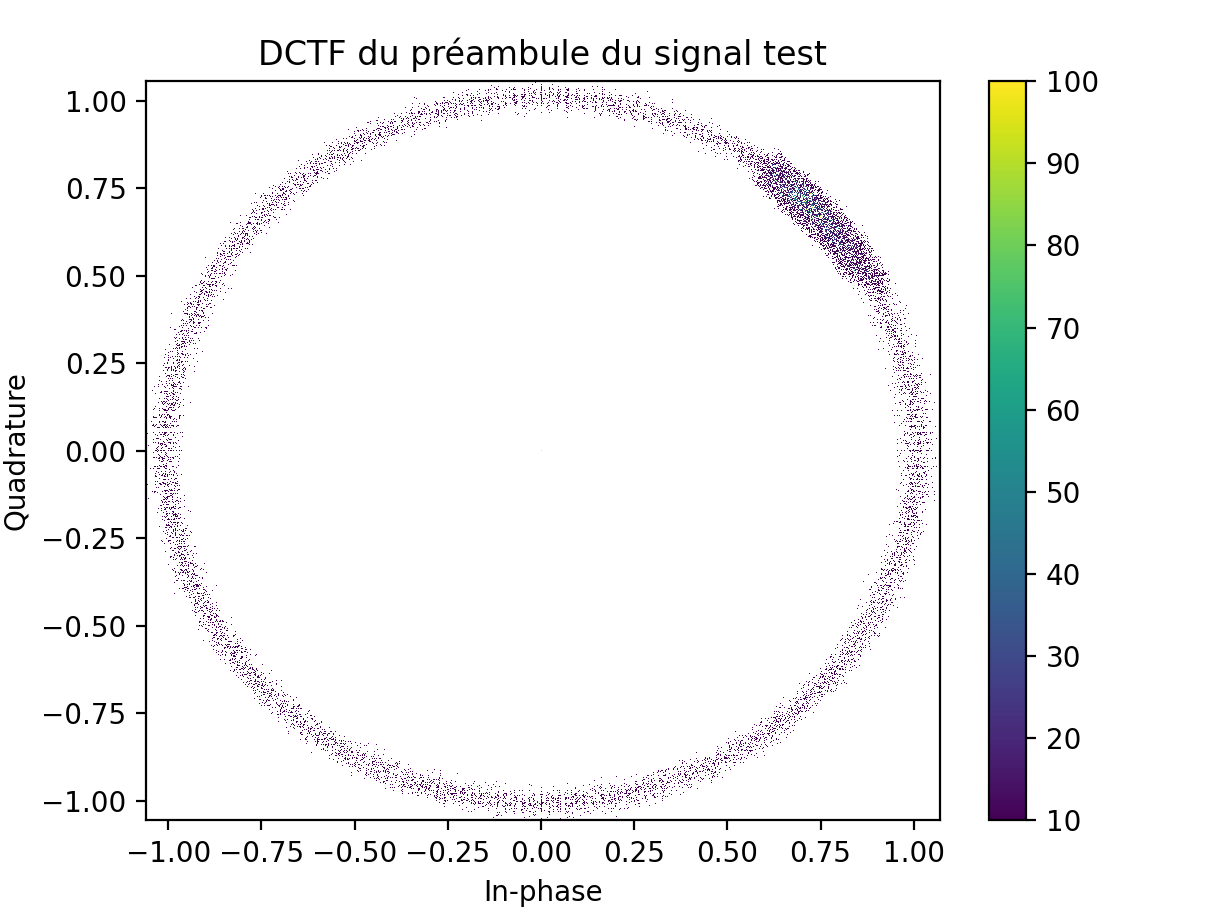
\includegraphics[scale=0.3]{images/dctf5.png}
\caption{DCTF du signal test}\label{term318}
\end{figure}

Maintenant que la région d'intérêt est indetifiée, il faut l'extraire. C'est ce qui sera extrait de cette DCTF qui sera la signature du signal, et donc permettra l'identification du module. Pour déterminer la meilleure valeur dans le plan à récuperer, la méthode suivante permet de récupérer le centre de la zone dense. La librairie Numpy de python permet de créer un histogramme en deux dimension de la DCTF. Afin d'extraire la valeur la plus pertinente (le centre de la zone dense), le point le plus dense de l'histogramme sert de référentiel. Sa valeur de densité est calculée (c'est à dire le nombre d'échantillons présent dans cette zone définie par l'histogramme). Afin de mieux refléter le centre de la zone dense, tous les points ayant une valeur de densité au moins égale à 90 pourcent (valeur choisie dans \cite{loraDCTF}) de la zone la plus dense sont également considérés. La figure \ref{term319} montre les points sélectionnés pour le signal test dans la DCTF. Le centre euclidien est calculé à partir des points éligibles, sa valeur est la signature du signal.


\begin{figure}[h]
\centering

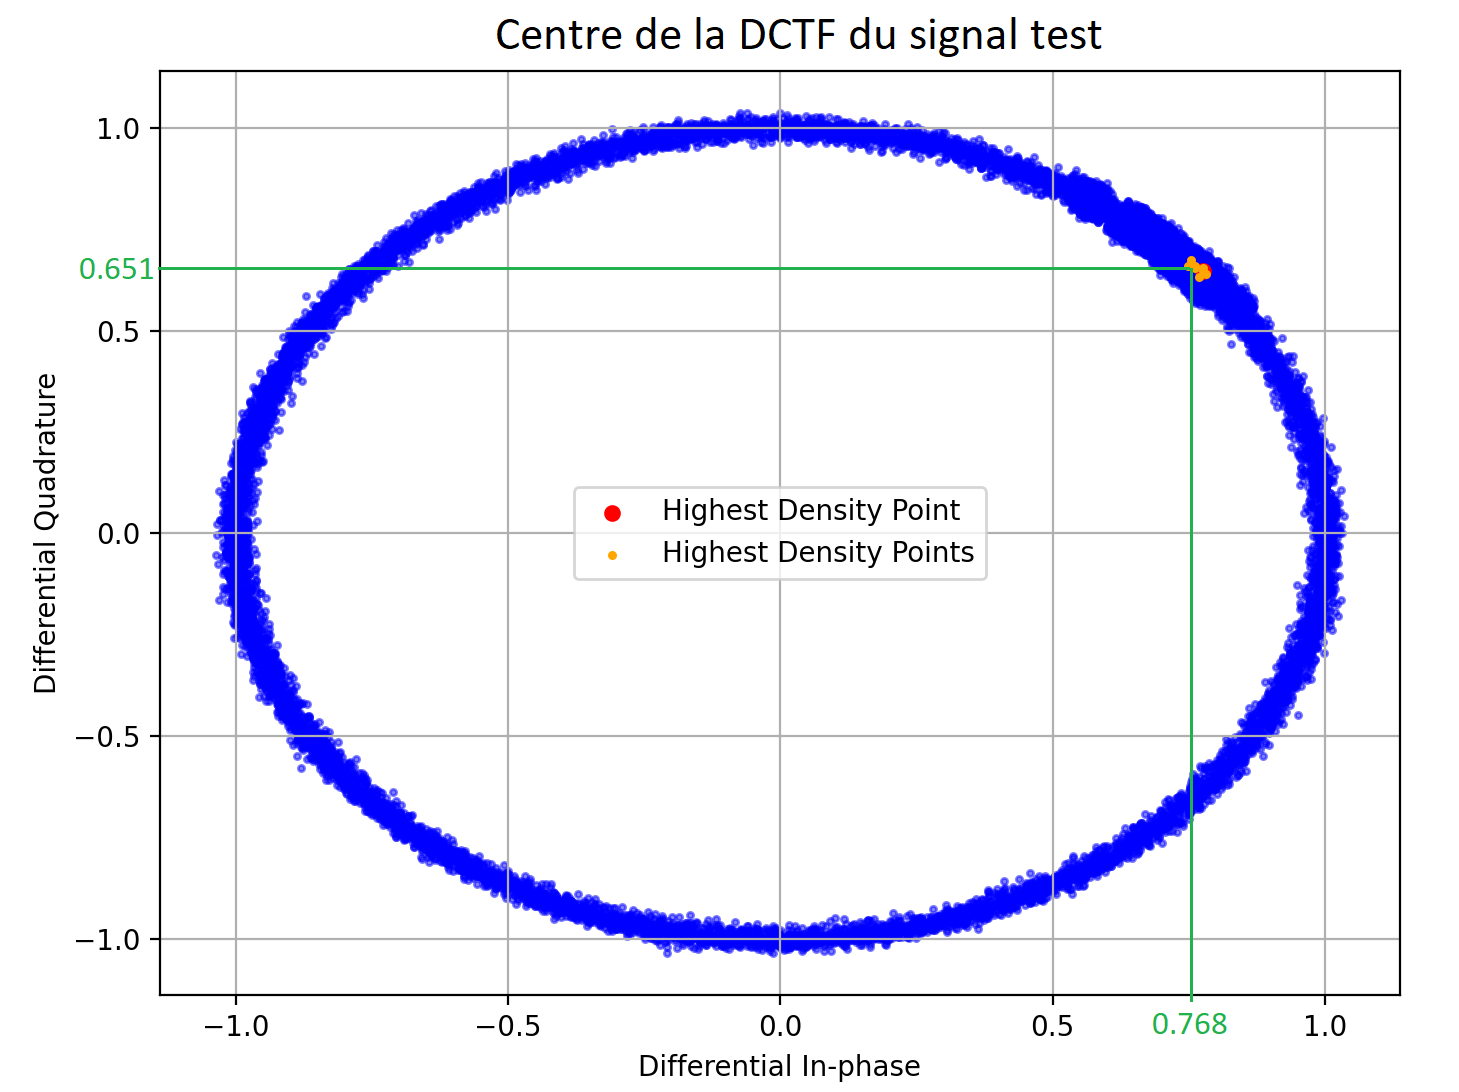
\includegraphics[scale=0.35]{images/dctf6.png}
\caption{Points de haute densité dans la DCTF du signal test}\label{term319}
\end{figure}


\section{Autres approches d'identification dans l'iot}\label{identification}

Comme tout appareil au sein d'un réseau, un appareil connecté dans l'iot possède de base différents moyens d'authentification. Son adresse MAC, son adresse IP, des informations relatives à sa manufacturation comme un numéro de série par example. De manière plus spécifiques, les noeuds au sein d'un réseau LoraWAN possède un DevEUI, un numéro unique accordé par le réseau à l'appareil. Cependant ses informations peuvent être compromises si appareils sont victimes de \textit{devices spoofing}, c'est à dire qu'un appareil malveillant usurpe l'indentité de sa cible, afin d'accéder au sein du réseau. D'autres attaques comme \textit{Man in The Middle} ou \textit{Replay attacks} peuvent également compromettre l'identité d'un appareil si on se base uniquement sur ses identifiant classiques\cite{attack}. Il faut donc pouvoir identifier les appareils mais sans se fier à leur informations. Il éxiste diverse méthodes basée sur différentes approches pour pouvoir indentifier un appareil. 

La première approche possible est de fier non pas à l'appareil directement ni aux données qu'il reçoit car celles ci pourraient également être compromises, mais à la routine sur sa communication. Cette approche, appelée \textit{Traffic related pattern} où s'intéresse au comportement d'un appareil au sein d'un réseau. L'article publié par H. Kawai, S. Ata et N. Nakamura \cite{pattern} propose notament d'analyser via machine learning le \textit{traffic pattern} c'est à dire le comportement du traffic.

Une autre approche s'intéresse à la position géographique d'un appareil. En effet il est possible de mesure la qualité de la réception d'un signal, le \textit{Received Signal strengh Indicator} ou RSSI. Un étude a été menée sur des appareils lora par M. Anjum, MA. Khan et SA. Hassan\cite{rssi}. L'article utilise le \textit{Path Loss} pour estimer le RSSI. Via machine learning ils sont capables de recréer un système de positionement permettant l'identification d'appareil Lora.
